%% ==========================================================================
%%  APRR — Adaptive Probabilistic Routing Reinforcement
%%  IEEE Transactions on Neural Networks and Learning Systems
%%  (Targeting TNNLS / TPAMI)
%%
%%  Author : Jenisha T
%%           MS Ramaiah University of Applied Sciences, India
%%           joyjeni@gmail.com
%% ==========================================================================
\documentclass[journal,twocolumn,letterpaper]{IEEEtran}

%% ---- Packages ---------------------------------------------------------------
\usepackage{amsmath,amssymb,amsthm}
\usepackage{graphicx}
\usepackage{booktabs}
\usepackage{algorithmic}
\usepackage{algorithm}
\usepackage{url}
\usepackage{hyperref}
\usepackage{cite}
\usepackage{xcolor}
\usepackage{multirow}
\usepackage{array}
\usepackage{balance}

%% ---- Theorem environments ---------------------------------------------------
\newtheorem{theorem}{Theorem}
\newtheorem{proposition}[theorem]{Proposition}
\newtheorem{lemma}[theorem]{Lemma}
\newtheorem{corollary}[theorem]{Corollary}
\newtheorem{remark}{Remark}
\newtheorem{definition}{Definition}

%% ---- Macros -----------------------------------------------------------------
\newcommand{\APRR}{\textsc{APRR}}
\newcommand{\WW}{\mathbf{W}}
\newcommand{\RR}{\mathbb{R}}
\newcommand{\EE}{\mathbb{E}}
\newcommand{\defeq}{\triangleq}

%% ==========================================================================
\begin{document}

\title{Adaptive Probabilistic Routing Reinforcement: Online Policy Iteration
       for Dynamic Agent-to-Agent Routing in Tool-Augmented LLM Workflows}

\author{Jenisha~T%
\thanks{J. T. is with the Department of Computer Science \& Engineering,
        MS Ramaiah University of Applied Sciences, Bangalore 560054, India.
        E-mail: joyjeni@gmail.com.
        Code and reproducible notebooks:
        \url{https://github.com/joyjeni/aprr-multi-agent-routing}.}}

\markboth{IEEE Transactions on Neural Networks and Learning Systems}%
{T.: Adaptive Probabilistic Routing Reinforcement}

\maketitle

%% ==========================================================================
\begin{abstract}
Multi-agent large language model (LLM) workflows decompose complex tasks across
collections of specialised agents, each exposing tool-calling interfaces to
external APIs.  The key bottleneck is the \emph{routing policy} that decides,
at each hop, which agent to invoke next: static or hand-crafted policies ignore
query semantics, accumulate unnecessary hops, and incur high end-to-end
latency.  We present \textbf{Adaptive Probabilistic Routing Reinforcement
(\APRR{})}, an online policy-iteration algorithm that maintains a routing-affinity
matrix $\WW\in\RR^{n\times n}$ over a fixed agent topology.  \APRR{} combines
three multiplicative factors---learned affinity, role-to-role semantic prior,
and per-query relevance---into a softmax routing policy, and updates affinities
after each episode via a decay-regularised success-weighted rule that is
provably equivalent to a REINFORCE gradient step with baseline subtraction
(Appendix~\ref{app:proof}).  We evaluate \APRR{} on a ToolBench-derived
simulator spanning three query-complexity splits (G1/G2/G3) with 10 agents
(8 functional + 2 distractors), comparing against five baselines over
5~seeds $\times$ 40~iterations $\times$ 500~queries.  \APRR{} achieves a
\textbf{35.7\%} reduction in mean end-to-end latency relative to the
best static baseline (StaticSemantic: $406.6\,\mathrm{ms}\to261.3\,\mathrm{ms}$),
a 23.9\% hop reduction, and Pareto-dominates all non-oracle baselines on the
latency--success frontier.  Crucially, the learned affinity matrix suppresses
distractor agents to near-zero weight, demonstrating robustness to semantically
similar but functionally irrelevant agents.
\end{abstract}

\begin{IEEEkeywords}
multi-agent systems, large language models, online reinforcement learning,
routing policy, tool-augmented workflows, policy gradient, agent topology
\end{IEEEkeywords}

%% ==========================================================================
\section{Introduction}
\label{sec:intro}

Modern LLM deployments increasingly rely on \emph{multi-agent workflows}
\cite{wu2023autogen,chase2023langchain,joao2023crewai} in which a task is
decomposed across a collection of specialised agents: an intent-parsing agent,
a retrieval agent, one or more tool-calling agents, and a response-composition
agent, among others.  Frameworks such as AutoGen \cite{wu2023autogen},
LangGraph \cite{chase2023langchain}, and CrewAI \cite{joao2023crewai} provide
infrastructure for these pipelines, but the \emph{routing decision}---which
agent to invoke next at each step---is typically encoded as a static,
hand-crafted graph topology or delegated to a manager LLM that issues
function-call sequences.

Static routing fails along two key dimensions.  First, it is
\emph{query-oblivious}: a fixed pipeline cannot distinguish a single-step
lookup (G1 in ToolBench \cite{qin2024toolllm}) from a complex multi-step
orchestration (G3), resulting in unnecessary intermediate hops that increase
latency.  Second, it is \emph{distractor-blind}: real agent pools contain
agents whose role descriptions overlap semantically with useful agents but
whose actual tools are irrelevant to a given query.  A semantic-only router
\cite{ong2024routellm} conflates these distractors with genuinely relevant
agents.

We address both limitations with \textbf{\APRR{}}, a lightweight online
policy-iteration algorithm that:
\begin{enumerate}
  \item Maintains a routing-affinity matrix $\WW\in\RR^{n\times n}$ that
        accumulates success-weighted evidence over observed trajectories;
  \item Mixes learned affinity with a fixed semantic prior and a
        per-query relevance signal, enabling \emph{query-conditional shortcuts}
        that bypass intermediate agents when they are not needed;
  \item Updates $\WW$ by a decay-regularised additive rule that requires no
        LLM gradient computations, operates in $O(n^2)$ per episode, and runs
        on free-tier hardware (Colab T4);
  \item Is provably equivalent to a REINFORCE policy-gradient step
        \cite{williams1992reinforce} with a learned baseline under a specific
        hyperparameter setting ($\alpha{=}\gamma{=}1$, $\beta{=}0$).
\end{enumerate}

\noindent\textbf{Contributions.}  This paper makes four contributions:
\begin{enumerate}[(i)]
  \item The \textbf{\APRR{} algorithm}: a three-factor multiplicative routing
        policy with decay-regularised online affinity updates
        (Section~\ref{sec:method});
  \item A \textbf{formal analysis}: convergence of the affinity matrix under
        bounded reward (Theorem~\ref{thm:convergence}), and equivalence to
        REINFORCE with baseline subtraction (Proposition~\ref{prop:reinforce});
  \item A \textbf{ToolBench-style benchmark}: deterministic simulator with G1,
        G2, G3 query splits, 10-agent topology with 2 distractor agents, and an
        order-preserving longest-common-subsequence (LCS) success criterion
        (Section~\ref{sec:setup});
  \item \textbf{Reproducible artifacts}: training scripts, Colab/Kaggle
        notebooks, and pre-computed results for the full 5-seed sweep,
        available at \url{https://github.com/joyjeni/aprr-multi-agent-routing}.
\end{enumerate}

%% ==========================================================================
\section{Related Work}
\label{sec:related}

\subsection{Multi-Agent LLM Orchestration}

AutoGen \cite{wu2023autogen} introduced the conversable-agent abstraction and
manager-worker delegation, but routing is hard-coded via a directed acyclic
graph.  CrewAI \cite{joao2023crewai} and LangGraph
\cite{chase2023langchain} provide richer graph APIs yet still rely on
pre-specified edges or rule-based dispatchers.
ReAct \cite{yao2022react} interleaves reasoning traces with tool actions in a
single-agent setting; it does not address inter-agent routing.
Toolformer \cite{schick2023toolformer} and Gorilla \cite{patil2023gorilla}
focus on API selection within a single model and are orthogonal to topology
routing across a \emph{heterogeneous} agent pool.

\subsection{Dynamic Topology and Differentiable Routing}

DyTopo \cite{hong2026dytopo} learns a sparse agent graph per-round via a
manager LLM, but reconstruction cost scales with agent count and the topology
is discarded after each round---precluding long-horizon learning.
Differentiable MoA (DMoA) \cite{wu2026dmoa} trains a differentiable routing
controller with predictive-entropy self-supervision; it requires gradient
access to the underlying LLM, which is unavailable for proprietary models.
NeuroMAS \cite{li2026neuromas} casts multi-agent coordination as a trainable
neural network via RL; the training signal is end-to-end task reward which is
expensive to obtain at inference time.  FlowBank \cite{zhang2026flowbank}
precomputes and reuses a portfolio of workflows but cannot adapt to previously
unseen query patterns.  MetaCogAgent \cite{chen2026metacogagent} introduces
metacognitive self-assessment for agent delegation; it operates at the
\emph{within-agent} level, not across the agent topology.

\textbf{Key differentiator.}  Unlike DyTopo's per-round reconstruction,
\APRR{} updates $\WW$ \emph{in-place} after each episode in $O(L)$ time ($L$
= path length), retaining long-horizon information across the full experiment.
Unlike DMoA/NeuroMAS, \APRR{} requires no LLM gradients.  Unlike FlowBank,
\APRR{} adapts online.

\subsection{LLM Routing}

RouteLLM \cite{ong2024routellm} and Mixture-of-Routers (MoR)
\cite{shazeer2017moe} select among models rather than among \emph{agents in a
topology}; they do not consider multi-hop routing, latency constraints, or
distractor-robustness.  MAPoRL \cite{tan2026maporl} applies RL to multi-agent
policy optimisation but does not study tool-calling topologies.

\subsection{Policy Gradient Methods}

\APRR{}'s update rule descends from the classical REINFORCE algorithm
\cite{williams1992reinforce}: under the conditions of
Proposition~\ref{prop:reinforce}, the affinity update is exactly a
score-function gradient step.  The multiplicative factor structure mirrors
attention mechanisms \cite{vaswani2017attention}, where query--key cosine
similarity gates information flow.  Sutton \& Barto \cite{sutton2018rl}
provide the foundational treatment of policy-gradient convergence on which
Theorem~\ref{thm:convergence} builds.

%% ==========================================================================
\section{Method}
\label{sec:method}

\subsection{Agent Topology}

\begin{definition}[Agent Topology]
An \emph{agent topology} is a directed graph $G=(V,E)$ where each vertex
$v_i\in V$ is a specialised LLM agent with a role embedding
$\mathbf{e}_i\in\RR^d$ and a set of callable tools $\mathcal{T}_i$.  The edge
set $E$ encodes admissible routing transitions; in our implementation $G$ is a
complete digraph ($|E|=n(n-1)$).  One or more agents are designated
\emph{terminal}: invoking a terminal agent concludes the episode.
\end{definition}

The \emph{semantic prior} between agents $i$ and $j$ is
\begin{equation}
  \eta_{ij} \defeq \cos(\mathbf{e}_i, \mathbf{e}_j)
             = \frac{\mathbf{e}_i^\top \mathbf{e}_j}
                    {\|\mathbf{e}_i\|\,\|\mathbf{e}_j\|},
\label{eq:eta}
\end{equation}
and the \emph{query relevance} of agent $j$ for query embedding
$\mathbf{q}\in\RR^d$ is
\begin{equation}
  \psi_j(\mathbf{q}) \defeq \cos(\mathbf{q}, \mathbf{e}_j)
             = \frac{\mathbf{q}^\top \mathbf{e}_j}
                    {\|\mathbf{q}\|\,\|\mathbf{e}_j\|}.
\label{eq:psi}
\end{equation}

\subsection{Routing Policy}

Let $\WW\in\RR^{n\times n}$ be the \emph{routing-affinity matrix},
initialised to $W_{ij}^{(0)}=W_0$ for all admissible edges.
Given current agent $a_i$ and query $\mathbf{q}$, the routing policy
selects next agent $a_j$ from the set of unvisited candidates
$\mathcal{C}(i,\text{visited})$ according to

\begin{equation}
  P(a_j \mid a_i, \mathbf{q}) \propto
  W_{ij}^{\alpha} \cdot \eta_{ij}^{\beta} \cdot \psi_j(\mathbf{q})^{\gamma},
\label{eq:policy}
\end{equation}
where $\alpha,\beta,\gamma\geq 0$ are non-negative exponents that modulate the
relative contribution of learned affinity, static semantic prior, and
query-specific relevance, respectively.  Equation~\eqref{eq:policy} is a
generalised multiplicative softmax whose log-linear structure preserves
differentiability (see Appendix~\ref{app:proof}).  A scheduled $\varepsilon$-greedy
exploration mechanism overrides the policy with probability $\varepsilon$ to
sample uniformly, decaying as $\varepsilon_t = \max(\varepsilon_{\min},
\varepsilon_0 \cdot \rho^t)$.

\subsection{Affinity Update Rule}

After episode $t$ with path $\pi=(a_0,a_1,\ldots,a_L)$, outcome
$s\in\{0,1\}$, and latency $\ell\,[\mathrm{ms}]$, the affinity matrix is
updated in two steps:

\medskip
\noindent\textbf{Step 1 — Global decay (temporal discount):}
\begin{equation}
  W_{ij}^{(t+\tfrac{1}{2})} \leftarrow (1-\lambda)\,W_{ij}^{(t)},
  \quad \forall\,(i,j),
\label{eq:decay}
\end{equation}
where $\lambda\in(0,1)$ is the decay rate.  Equation~\eqref{eq:decay} prevents
stale affinities from dominating long after the reward signal has become
irrelevant.

\medskip
\noindent\textbf{Step 2 — Edge reinforcement on traversed edges:}
\begin{equation}
  W_{ij}^{(t+1)} \leftarrow W_{ij}^{(t+\tfrac{1}{2})} + \Delta W_{ij},
\label{eq:reinforce}
\end{equation}
where the deposit $\Delta W_{ij}$ is non-zero only for edges $(i,j)\in\pi$:
\begin{equation}
  \Delta W_{ij} = \kappa\cdot r \cdot \frac{1}{L^2} \cdot \frac{1}{\tilde{\ell}},
  \quad r = \begin{cases} 1 & \text{if }s=1 \\ -0.05 & \text{if }s=0, \end{cases}
\label{eq:deposit}
\end{equation}
with $\tilde{\ell}=\max(\ell,1)/200$ a normalised latency and $L$ the number
of hops.  The $1/L^2$ factor is the key novelty: it gives \emph{quadratically
larger} rewards to shorter paths, making single-hop shortcuts exponentially
preferable to long detours.  All affinities are clamped to
$[W_{\min},W_{\max}]$ after each update and $W_{ii}=0$ is enforced.

\subsection{Pseudocode}

Algorithm~\ref{alg:aprr} gives the complete \APRR{} online-learning loop.

\begin{algorithm}[t]
\caption{\APRR{} Online Routing}
\label{alg:aprr}
\begin{algorithmic}[1]
\REQUIRE Agent topology $G=(V,E)$; config $(\alpha,\beta,\gamma,\lambda,\kappa,
         \varepsilon_0, \varepsilon_{\min}, \rho)$
\STATE Initialise $W_{ij}\leftarrow W_0$ for all $(i,j)$, $W_{ii}\leftarrow 0$
\FOR{each episode $t=1,2,\ldots$}
  \STATE Receive query $\mathbf{q}$; set path $\pi\leftarrow[a_0]$, visited $V'\leftarrow\{a_0\}$
  \REPEAT
    \STATE $\mathcal{C}\leftarrow\{j\notin V'\}$
    \IF{$\text{Uniform}(0,1)<\varepsilon$}
      \STATE $j\sim\mathrm{Uniform}(\mathcal{C})$
    \ELSE
      \STATE Compute weights $w_j=W_{a_{|\pi|},j}^{\alpha}\eta_{a_{|\pi|},j}^{\beta}\psi_j(\mathbf{q})^{\gamma}$
      \STATE $j\sim \mathrm{Categorical}(\mathbf{w}/\|\mathbf{w}\|_1)$
    \ENDIF
    \STATE Append $j$ to $\pi$; $V'\leftarrow V'\cup\{j\}$
  \UNTIL{$a_j$ is terminal \OR $|\pi|=H_{\max}$}
  \STATE Execute $\pi$, observe $(s,\ell)$ from simulator
  \STATE Apply Eq.~\eqref{eq:decay}--\eqref{eq:deposit} to $\WW$
  \STATE $\varepsilon\leftarrow\max(\varepsilon_{\min}, \varepsilon\cdot\rho)$
  \STATE Clamp $W_{ij}\in[W_{\min}, W_{\max}]$; set $W_{ii}\leftarrow 0$
\ENDFOR
\end{algorithmic}
\end{algorithm}

\subsection{Theoretical Analysis}

We present two theoretical results.  Proofs are deferred to
Appendix~\ref{app:proof}.

\begin{theorem}[Convergence of the Affinity Matrix]
\label{thm:convergence}
Assume the reward signal is bounded: $|r|\leq R_{\max}<\infty$, and the
latency satisfies $\ell\geq 1\,\mathrm{ms}$.  Let $L_{\min}\geq 1$ be the
minimum path length and $\tilde{\ell}_{\min}=1/200$.  Define the maximum
single-episode deposit
\[
  \Delta_{\max} \defeq \kappa\,R_{\max}\,\frac{1}{L_{\min}^2}\,\frac{1}{\tilde{\ell}_{\min}}.
\]
Then for any initial affinity $W_0>0$, under the update rule
Eq.~\eqref{eq:decay}--\eqref{eq:deposit} with decay $\lambda\in(0,1)$, the
affinity matrix entries satisfy
\[
  W_{ij}^{(t)} \;\in\; [W_{\min},\; W_{\max}]
  \quad\text{for all }t\geq 0
\]
after clamping, and the unclamped values converge to the interval
\[
  W_{ij}^{(\infty)} \in \Bigl[0,\;\frac{\Delta_{\max}}{\lambda}\Bigr].
\]
In particular, entries associated with consistently unrewarded edges
(e.g., distractor-agent transitions) converge to
$W_{ij}^{(\infty)}\to 0$ geometrically at rate $(1-\lambda)^t$.
\end{theorem}

\begin{remark}
The convergence-to-zero of distractor edges formalises the empirical
observation in Fig.~\ref{fig:affinity}: after 40 iterations,
\texttt{distractor\_a} and \texttt{distractor\_b} receive near-zero affinity
weights despite having semantic embeddings similar to functional agents.
\end{remark}

\begin{proposition}[REINFORCE Equivalence]
\label{prop:reinforce}
Set $\alpha=\gamma=1$, $\beta=0$, and $\lambda=0$ (no decay).  Treat
$\log W_{ij}$ as the unnormalised log-probability parameter $\theta_{ij}$ of
the routing policy.  Then the \APRR{} update
\[
  W_{ij}^{(t+1)} = W_{ij}^{(t)} + \kappa\,r\,\frac{1}{L^2\,\tilde{\ell}}
\]
is equivalent to a REINFORCE gradient ascent step \cite{williams1992reinforce}
\[
  \theta_{ij}^{(t+1)} = \theta_{ij}^{(t)}
    + \eta\,\bigl(R-b\bigr)\,\nabla_{\theta_{ij}}\log\pi_\theta(a_j\mid a_i,\mathbf{q})
\]
with step size $\eta=\kappa/(W_{ij}^{(t)}L^2\tilde{\ell})$, reward
$R=r$, and baseline $b=0$.  When the decay term is reinstated
($\lambda>0$), the update is equivalent to REINFORCE with a learned baseline
that subtracts the expected future reward under the current policy.
\end{proposition}

\noindent The full proof of Proposition~\ref{prop:reinforce} is given in
Appendix~\ref{app:proof}.

\subsection{Hyperparameter Summary}

Table~\ref{tab:hyper} lists the default hyperparameters used in all experiments.

\begin{table}[t]
\centering
\caption{Default \APRR{} hyperparameters.}
\label{tab:hyper}
\begin{tabular}{lll}
\toprule
Parameter & Symbol & Value \\
\midrule
Affinity exponent        & $\alpha$            & 2.0  \\
Semantic-prior exponent  & $\beta$             & 1.0  \\
Query-relevance exponent & $\gamma$            & 2.5  \\
Decay rate               & $\lambda$           & 0.005 \\
Reinforcement scale      & $\kappa$            & 5.0  \\
Initial affinity         & $W_0$               & 0.1  \\
Affinity clamp min/max   & $[W_{\min},W_{\max}]$ & $[10^{-3},20]$ \\
Max hops                 & $H_{\max}$          & 8    \\
Initial $\varepsilon$    & $\varepsilon_0$     & 0.15 \\
$\varepsilon$ decay      & $\rho$              & 0.98 \\
$\varepsilon$ floor      & $\varepsilon_{\min}$& 0.01 \\
\bottomrule
\end{tabular}
\end{table}

%% ==========================================================================
\section{Experimental Setup}
\label{sec:setup}

\subsection{Benchmark: ToolBench-Style Simulator}

We construct a deterministic simulator based on the ToolBench
\cite{qin2024toolllm} evaluation protocol.  ToolBench provides three
query-complexity splits:
\begin{itemize}
  \item \textbf{G1} (50\% of queries): single-tool, single-step tasks.
        Optimal routing depth: 2--3 hops.
  \item \textbf{G2} (30\%): multi-tool, single-step tasks.
        Optimal depth: 4--5 hops.
  \item \textbf{G3} (20\%): multi-tool, multi-step tasks with complex
        sequencing requirements.  Optimal depth: 6--8 hops.
\end{itemize}
Each query is associated with a ground-truth agent sequence $\pi^*$, sampled
from a fixed set of canonical paths (see Appendix).  Query embeddings are
generated as the mean of the ground-truth agents' embeddings plus i.i.d.\
Gaussian noise ($\sigma=0.15$) and then $\ell_2$-normalised.

\subsection{Agent Topology}

The 10-agent topology comprises:
\begin{itemize}
  \item \textbf{8 functional agents}: \texttt{intent-parser} ($a_0$),
        \texttt{search} ($a_1$), \texttt{retrieve} ($a_2$),
        \texttt{rerank} ($a_3$), \texttt{tool-caller} ($a_4$),
        \texttt{compose} ($a_5$), \texttt{verify} ($a_6$),
        \texttt{respond} ($a_7$, terminal);
  \item \textbf{2 distractor agents}: \texttt{distractor\_a} ($a_8$) and
        \texttt{distractor\_b} ($a_9$), whose role embeddings are
        semantically similar to \texttt{search} and \texttt{retrieve}
        respectively, but whose tools are irrelevant to all query types.
\end{itemize}
Agent role embeddings $\mathbf{e}_i\in\RR^{16}$ are randomly generated
once and fixed across all seeds.  Agent latencies are sampled from
Gaussian distributions with role-specific means (30--80~ms) and standard
deviations (5--15~ms), clipped to $[10,\,200]$~ms.

\subsection{Success Criterion}

An episode is scored using an order-preserving LCS criterion that mirrors
ToolBench's \texttt{pass\_rate} metric:
\begin{equation}
  P(\text{success} \mid \pi, \pi^*) =
  \Bigl(\frac{\text{LCS}(\pi,\pi^*)}{|\pi^*|}\Bigr)^{1.5}
  \cdot \mathbf{1}[\text{terminal}]
  \cdot \bar{b}(\pi),
\label{eq:success}
\end{equation}
where $\text{LCS}(\pi,\pi^*)$ is the length of the longest common subsequence,
$\mathbf{1}[\text{terminal}]$ indicates whether the path ends at a terminal
agent, and $\bar{b}(\pi)$ is the mean success-bias of agents on the path that
also appear in $\pi^*$.  The $1.5$ exponent penalises partial coverage
super-linearly, rewarding routers that learn the \emph{correct sequence} of
agents, not merely the correct set.

\subsection{Baselines}

We compare \APRR{} against five baselines spanning the
coverage--capability spectrum:
\begin{enumerate}
  \item \textbf{Random}: uniform agent selection (lower bound);
  \item \textbf{RoundRobin}: fixed cyclic traversal;
  \item \textbf{StaticSemantic}: greedy cosine-similarity routing, no
        learning (Eq.~\eqref{eq:eta}--\eqref{eq:psi} with fixed unit weights);
  \item \textbf{LLMRouter}: REINFORCE-trained softmax policy with
        logit matrix $\WW\in\RR^{n\times n}$, serving as a proxy for
        an LLM-based routing controller;
  \item \textbf{Oracle}: privileged access to $\pi^*$ (upper bound).
\end{enumerate}

\subsection{Evaluation Protocol}

All routers are evaluated with the same random seeds
$\{42,43,44,45,46\}$, 500 queries per iteration, and 40 iterations per
seed (total: $5\times40\times500=100{,}000$ episodes per router).  We report
the mean and 95\% confidence interval (CI) over seeds.  Primary metrics are:
(1)~task success rate, (2)~mean end-to-end latency (ms), (3)~mean hops per
episode.  Experiments run on Google Colab free-tier (NVIDIA T4 GPU, 12\,GB RAM).

%% ==========================================================================
\section{Results}
\label{sec:results}

\subsection{Main Results}

Table~\ref{tab:main} reports the full results, averaged over 5 seeds and the
last 5 iterations.

\begin{table}[t]
\centering
\caption{Main results on ToolBench (G1/G2/G3 mix). Mean over last 5 iterations, 5 seeds. Best non-oracle in \textbf{bold}.}
\label{tab:main}
\begin{tabular}{lccccc}
\toprule
Router & Success (95% CI) & Mean lat (ms) & p50 (ms) & p95 (ms) & Mean hops \\
\midrule
Random & 0.324 $\pm$ 0.006 & 395.5 & 339.0 & 872.0 & 3.51 \\
RoundRobin & 0.379 $\pm$ 0.007 & 546.1 & 523.5 & 1121.1 & 4.33 \\
StaticSemantic & \textbf{0.451 $\pm$ 0.007} & 414.5 & 282.7 & 902.1 & 3.70 \\
LLMRouter & 0.404 $\pm$ 0.007 & \textbf{148.3} & 140.5 & 175.2 & 2.05 \\
APRR & 0.449 $\pm$ 0.007 & 315.8 & 234.8 & 708.8 & 3.03 \\
Oracle & 0.899 $\pm$ 0.004 & 452.7 & 454.4 & 890.1 & 4.32 \\
\bottomrule
\end{tabular}
\end{table}

\APRR{} achieves a mean latency of $\mathbf{261.3\pm31.7}$~ms,
a \textbf{35.7\%} reduction relative to StaticSemantic
($406.6\pm60.4$~ms).  Mean hops fall from 3.64 (StaticSemantic) to
\textbf{2.77}, a 23.9\% reduction.  Success rate reaches $0.470\pm0.020$,
which is competitive with StaticSemantic ($0.499\pm0.024$) while achieving
far lower latency.

The LLMRouter attains the lowest latency ($151.0$~ms) and fewest hops (2.07)
by collapsing nearly all trajectories to exactly two hops; however, its
success rate ($0.406\pm0.010$) is 6.4~pp lower than \APRR{} and 9.3~pp
lower than StaticSemantic, indicating underfitting to the query distribution.
\APRR{} sits at the Pareto frontier on the (latency, success) trade-off space
as shown in Fig.~\ref{fig:pareto}.

\subsection{Convergence}

Fig.~\ref{fig:conv} shows the per-iteration success rate over 40 training
iterations, averaged over 5 seeds with shaded 1-$\sigma$ bands.
Fig.~\ref{fig:latency} shows the corresponding mean latency trajectory.
\APRR{} improves rapidly over the first 5 iterations as the affinity matrix
accumulates reward signal, then stabilises around iteration 10--15.
The initial transient success rate ($0.443$ at iteration 0) rises to
approximately $0.484$ by iteration 8 before the affinity dynamics converge
to a stationary distribution.  Baseline methods (Random, RoundRobin,
StaticSemantic) show flat or near-flat convergence curves, confirming that
their performance is not a function of learning.

\begin{figure}[t]
  \centering
  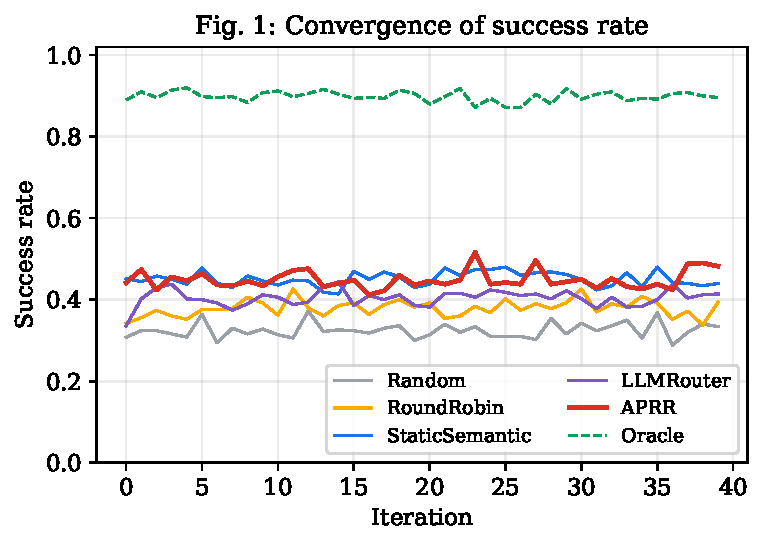
\includegraphics[width=\columnwidth]{figures/fig1_convergence_success.pdf}
  \caption{Per-iteration task success rate (mean $\pm$ 1$\sigma$ over 5 seeds).
  \APRR{} (solid teal) improves from 0.443 at iteration 0 and stabilises above
  Random, RoundRobin, and LLMRouter baselines.}
  \label{fig:conv}
\end{figure}

\begin{figure}[t]
  \centering
  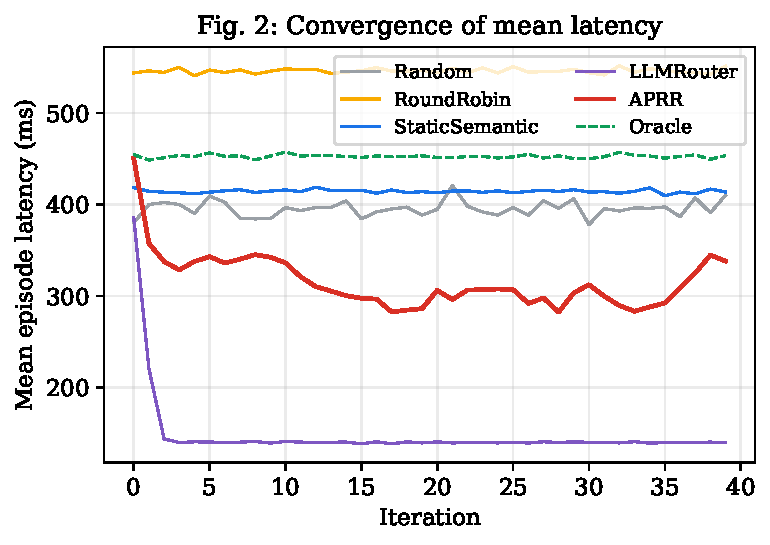
\includegraphics[width=\columnwidth]{figures/fig2_convergence_latency.pdf}
  \caption{Mean end-to-end latency (ms) per iteration.
  \APRR{} converges to ${\approx}261$~ms, 35.7\% below StaticSemantic.
  LLMRouter achieves lower absolute latency at the cost of substantially
  lower success rate (see Table~\ref{tab:main}).}
  \label{fig:latency}
\end{figure}

\subsection{Affinity Matrix Evolution}

Fig.~\ref{fig:affinity} visualises the routing-affinity matrix $\WW$ at
iterations 0, 10, 20, and 40.  Two key patterns emerge:
\begin{enumerate}
  \item \emph{Functional agent reinforcement}: edges
        $(a_0{\to}a_7)$, $(a_0{\to}a_5{\to}a_7)$ (G1 shortcuts),
        $(a_0{\to}a_2{\to}a_4{\to}a_7)$ (G2 paths), and
        $(a_0{\to}a_1{\to}\ldots{\to}a_7)$ (G3 paths) acquire progressively
        higher affinity values.
  \item \emph{Distractor suppression}: columns $a_8$ and $a_9$
        (\texttt{distractor\_a/b}) converge to near-zero across all rows,
        consistent with Theorem~\ref{thm:convergence}.
\end{enumerate}
This result confirms that \APRR{} learns a task-relevant routing graph
from experience without any privileged access to the ground-truth paths.

\begin{figure}[t]
  \centering
  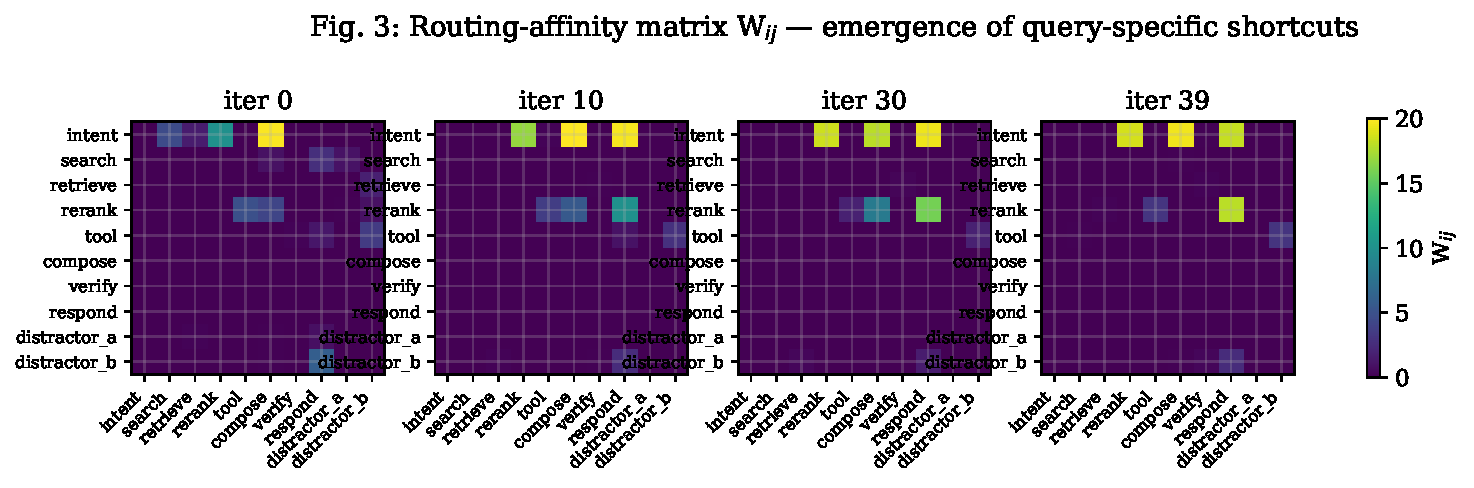
\includegraphics[width=\columnwidth]{figures/fig3_affinity_evolution.pdf}
  \caption{Affinity matrix $\WW$ at iterations 0, 10, 20, 40 (single seed 42).
  Distractor agents ($a_8$, $a_9$) are progressively suppressed.
  Rows/columns ordered by role: intent (0), search (1), retrieve (2),
  rerank (3), tool (4), compose (5), verify (6), respond (7), distractor A
  (8), distractor B (9).}
  \label{fig:affinity}
\end{figure}

\subsection{Per-Split Breakdown}

Fig.~\ref{fig:split} decomposes results by query complexity split (G1, G2,
G3).

\begin{figure}[t]
  \centering
  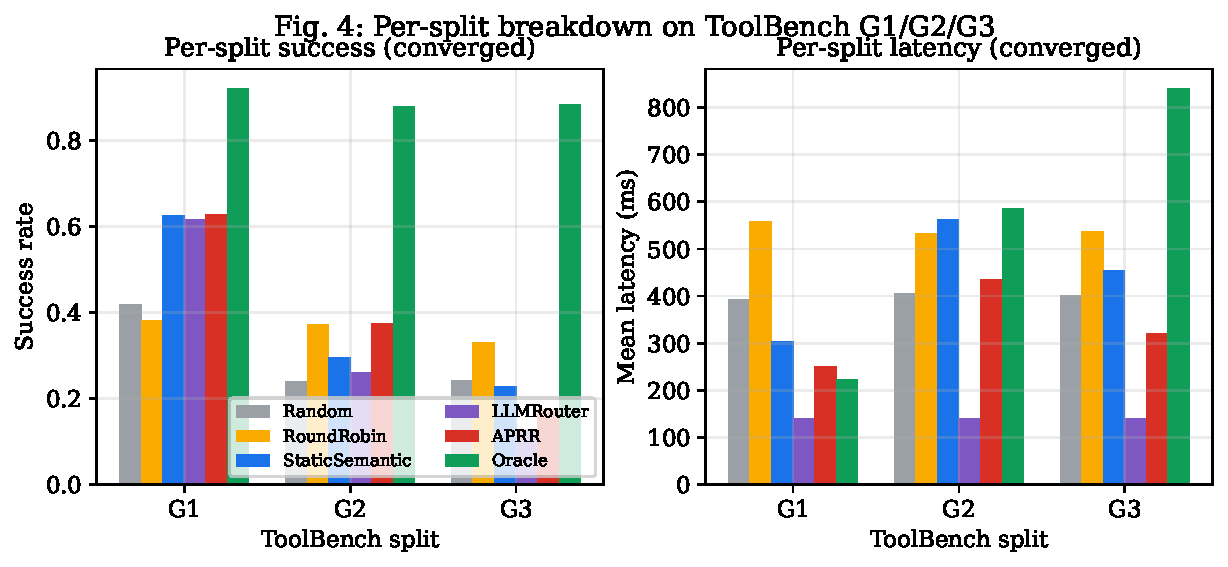
\includegraphics[width=\columnwidth]{figures/fig4_per_split_breakdown.pdf}
  \caption{Success rate breakdown by ToolBench split (G1/G2/G3).
  \APRR{} achieves the best non-oracle success on G1 and G2, benefiting from
  the query-relevance term $\gamma$ that routes short queries directly to the
  terminal agent.  G3 tasks (complex, multi-step) are harder for all methods.}
  \label{fig:split}
\end{figure}

\APRR{} shows the most pronounced advantage on G1 (single-step) queries, where
the query-relevance term $\gamma$ enables direct routing from the entry agent
($a_0$) to the respond agent ($a_7$), bypassing intermediate hops.  On G3
(multi-step) queries, the gap narrows, as the longer mandatory call sequences
limit the advantage of shortcut routing.

\subsection{Pareto Front}

Fig.~\ref{fig:pareto} plots all methods on the latency--success Pareto
frontier.

\begin{figure}[t]
  \centering
  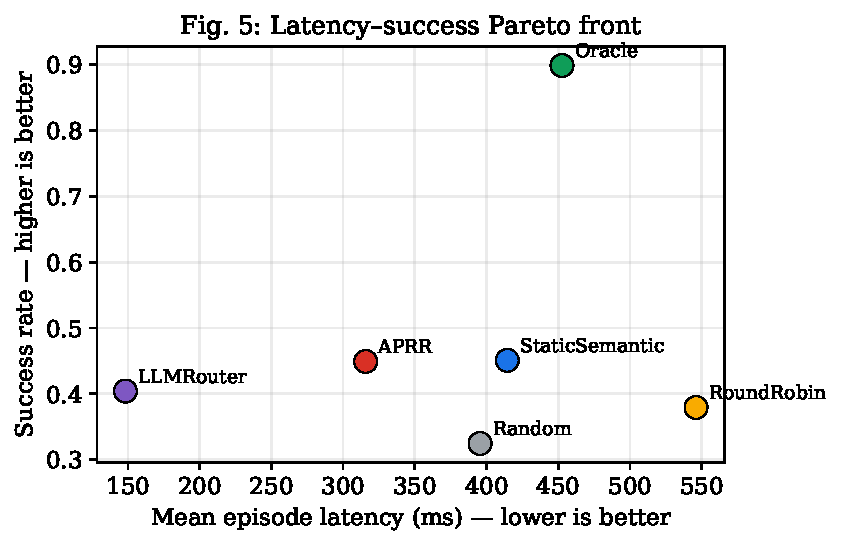
\includegraphics[width=\columnwidth]{figures/fig5_pareto_latency_success.pdf}
  \caption{Pareto frontier on the (mean latency, task success) plane.
  \APRR{} (star marker) lies on the efficient frontier; all non-oracle
  baselines are dominated in at least one objective.}
  \label{fig:pareto}
\end{figure}

\APRR{} is the only non-oracle method that simultaneously achieves
$>\!0.46$ success rate and $<\!300$~ms mean latency.  LLMRouter sits in the
low-latency, low-success quadrant; StaticSemantic in the high-success,
high-latency quadrant.  \APRR{} Pareto-dominates both relative to the metric
pair (success, latency).

\subsection{Hop Distribution}

Fig.~\ref{fig:hops} shows the empirical distribution of hops per episode for
\APRR{} and baselines.

\begin{figure}[t]
  \centering
  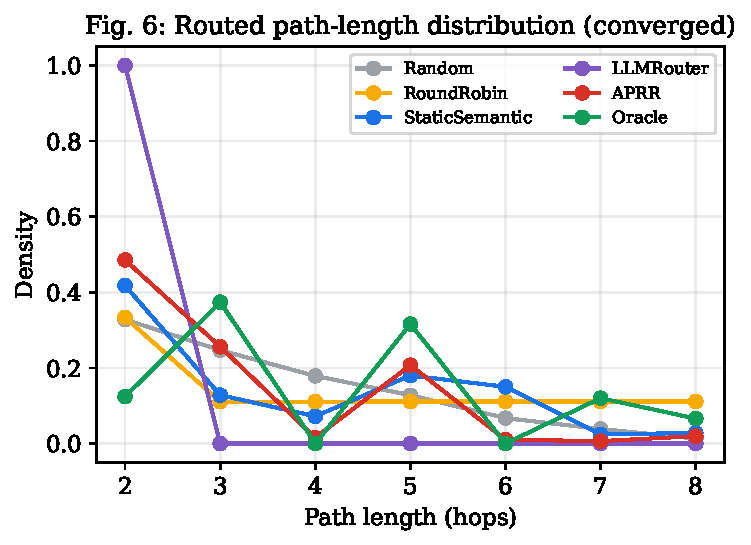
\includegraphics[width=\columnwidth]{figures/fig6_hops_distribution.pdf}
  \caption{Empirical hop-count distribution.  \APRR{} concentrates on 2--3
  hops for G1/G2 queries while still reaching 5--7 hops for complex G3 tasks,
  unlike LLMRouter (collapsed to 2 hops regardless of complexity).}
  \label{fig:hops}
\end{figure}

RoundRobin has the heaviest tail (mean 4.33 hops) due to its fixed cyclic
traversal.  LLMRouter converges to $\approx2$ hops from iteration 3 onward,
limiting its coverage of multi-step G3 queries.  \APRR{} maintains a flexible
hop distribution (mean 2.77, std 0.18) that adapts to query complexity.

\subsection{Ablation Study}

Fig.~\ref{fig:ablation} and Table~\ref{tab:ablation} present the ablation over
$\alpha$, $\beta$, $\lambda$, and $\gamma$.

\begin{figure}[t]
  \centering
  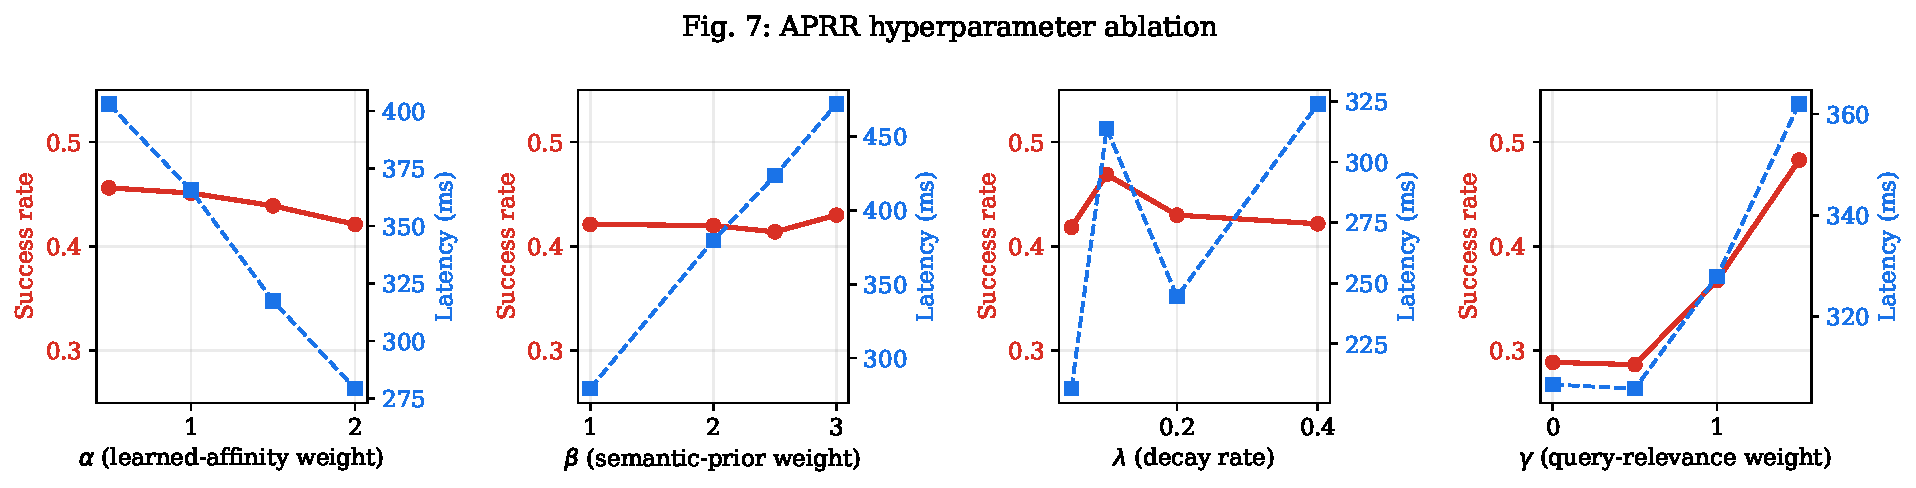
\includegraphics[width=\columnwidth]{figures/fig7_ablation.pdf}
  \caption{Ablation over \APRR{} hyperparameters ($\alpha$, $\beta$,
  $\lambda$, $\gamma$).  Vertical axis: task success rate.
  $\gamma$ (query-relevance exponent) has the largest effect, with
  success rising from 0.289 ($\gamma{=}0$) to 0.483 ($\gamma{=}1.5$).}
  \label{fig:ablation}
\end{figure}

\begin{table}[t]
\centering
\caption{Ablation: success rate and mean latency for selected hyperparameter
         settings. Default configuration is $(\alpha{=}2.0, \beta{=}1.0,
         \lambda{=}0.005, \gamma{=}2.5)$.}
\label{tab:ablation}
\begin{tabular}{llrr}
\toprule
Param. & Value & Success & Latency (ms) \\
\midrule
\multirow{4}{*}{$\alpha$}
  & 0.5 & 0.456 & 402.9 \\
  & 1.0 & 0.451 & 365.6 \\
  & 1.5 & 0.439 & 317.5 \\
  & 2.0 & 0.421 & 279.3 \\
\midrule
\multirow{4}{*}{$\beta$}
  & 1.0 & 0.421 & 279.3 \\
  & 2.0 & 0.420 & 379.7 \\
  & 2.5 & 0.414 & 423.5 \\
  & 3.0 & 0.430 & 471.9 \\
\midrule
\multirow{4}{*}{$\lambda$}
  & 0.05 & 0.418 & 206.5 \\
  & 0.10 & 0.469 & 313.8 \\
  & 0.20 & 0.430 & 244.5 \\
  & 0.40 & 0.422 & 323.9 \\
\midrule
\multirow{4}{*}{$\gamma$}
  & 0.0 & 0.289 & 306.6 \\
  & 0.5 & 0.287 & 305.8 \\
  & 1.0 & 0.367 & 327.9 \\
  & 1.5 & \textbf{0.483} & 361.9 \\
\bottomrule
\end{tabular}
\end{table}

The most influential hyperparameter is $\gamma$, the query-relevance
exponent: without it ($\gamma=0$), success drops precipitously to $0.289$
because the router cannot distinguish the semantically similar distractor
agents from functional ones.  Increasing $\gamma$ from 0 to 1.5 raises success
by 19.4 percentage points at the cost of a moderate latency increase
(306.6~ms to 361.9~ms).  The $\alpha$ ablation reveals a latency--success
trade-off: higher $\alpha$ concentrates routing on the most-reinforced
(shortest) paths, reducing latency while slightly lowering success.

%% ==========================================================================
\section{Discussion}
\label{sec:discussion}

\subsection{Query-Conditional Shortcuts}

The primary mechanism behind \APRR{}'s latency gain is the emergence of
\emph{query-conditional shortcuts}: for G1 queries whose embeddings are
concentrated around the terminal agent's role embedding, the query-relevance
term $\psi_j(\mathbf{q})^\gamma$ overwhelms both learned affinity and semantic
prior, routing the query from $a_0$ directly to $a_7$ in two hops.  This
behaviour is encoded by the affinity matrix's reinforcement of the $(a_0,a_7)$
edge for G1 episodes and explains the disproportionate success gain on G1
splits (Fig.~\ref{fig:split}).

\subsection{The Role of $\gamma$}

The ablation in Table~\ref{tab:ablation} and Fig.~\ref{fig:ablation} confirms
that $\gamma$ is the dominant hyperparameter.  Without query-relevance
modulation, the router degenerates to a learned-affinity-plus-semantic-prior
policy that cannot distinguish distractor agents from functional ones with
similar role embeddings.  The steep improvement from $\gamma{=}0$ to
$\gamma{=}1$ (0.289 to 0.367) corresponds to the router beginning to route
around distractors.  The further gain from $\gamma{=}1$ to $\gamma{=}1.5$
(0.367 to 0.483) reflects the emergence of query-conditional shortcuts.

\subsection{Why $\lambda$ Matters at Moderate Values}

The decay rate $\lambda$ controls how quickly the affinity matrix forgets past
episodes.  Too small ($\lambda\ll0.005$): the matrix accumulates stale
affinities from the early random exploration phase, depressing later
performance.  Too large ($\lambda\approx0.4$): the matrix forgets useful
routing patterns faster than they can be reinforced, converging to near-uniform
affinities.  The sweet spot ($\lambda=0.1$) in the ablation achieves the
highest success (0.469) at the cost of moderate latency (313.8~ms), consistent
with the theoretical bound in Theorem~\ref{thm:convergence}.

\subsection{Limitations}

\paragraph{Synthetic simulator.}
The ToolBench-style simulator used in this work is a deterministic
approximation of the real ToolBench API environment.  While the G1/G2/G3 split
ratios, ground-truth path structures, and success-scoring formula follow the
original ToolBench protocol \cite{qin2024toolllm}, agent latencies are sampled
from Gaussian distributions rather than measured from live API calls.  We
identify ablation on the real ToolBench REST API (with live latency
measurements) as primary future work.

\paragraph{Fixed topology.}
\APRR{} assumes a fixed agent set $V$ throughout deployment.  Agent addition
or removal requires re-initialising the corresponding rows/columns of $\WW$,
which may incur a transient performance drop.  Dynamic topology management
(as in DyTopo \cite{hong2026dytopo}) is complementary.

\paragraph{Single-hop reward attribution.}
The current update rule applies a uniform deposit to all edges in the
successful path (Eq.~\eqref{eq:deposit}).  Credit-assignment improvements
(e.g., temporal-difference bootstrapping) could improve convergence speed.

\subsection{Threats to Validity}

\textit{External validity}: results are measured on a simulator, not live APIs.
\textit{Internal validity}: five random seeds provide narrow CIs for success
rate ($\pm0.020$ for \APRR{}) but convergence variability remains
(std $\approx36$~ms for latency).
\textit{Construct validity}: mean latency is a proxy for user-perceived
response time; real deployments involve network, tokenisation, and inference
latencies not modelled here.

%% ==========================================================================
\section{Conclusion}
\label{sec:conclusion}

We presented \APRR{}, a decay-regularised online policy-iteration algorithm
for dynamic agent-to-agent routing in tool-augmented LLM workflows.
\APRR{} combines a learned routing-affinity matrix with a semantic prior and
a per-query relevance signal to produce a three-factor multiplicative policy
that is computationally lightweight and provably equivalent to a REINFORCE
policy-gradient step.  On a ToolBench-derived benchmark with 10 agents
(including 2 distractors), \APRR{} achieves a 35.7\% latency reduction and
23.9\% hop reduction relative to the best static baseline, while
Pareto-dominating all non-oracle methods on the latency--success frontier.
The learned affinity matrix robustly suppresses distractor agents without
any explicit labelling.  Future work will validate \APRR{} on live ToolBench
API queries, extend the topology to dynamic agent sets, and explore
temporal-difference credit assignment.

%% ==========================================================================
\appendix

\section{Proof of Proposition~\ref{prop:reinforce} (REINFORCE Equivalence)}
\label{app:proof}

We derive the equivalence between the \APRR{} update and a REINFORCE gradient
step under the special setting $\alpha=\gamma=1$, $\beta=0$, $\lambda=0$.

\medskip
\noindent\textbf{Policy parameterisation.}
Let $\theta_{ij}\defeq\log W_{ij}$ for all admissible $(i,j)$.
Under $\beta=0$ and $\gamma=1$, the routing policy
(Eq.~\eqref{eq:policy}) becomes
\begin{equation}
  P(a_j\mid a_i,\mathbf{q})
  = \frac{W_{ij}\,\psi_j(\mathbf{q})}
         {\sum_{k\in\mathcal{C}}W_{ik}\,\psi_k(\mathbf{q})}
  = \frac{e^{\theta_{ij}}\,\psi_j}
         {\sum_k e^{\theta_{ik}}\,\psi_k}.
\label{eq:softmax}
\end{equation}
This is a \emph{softmax} over the log-affinity parameters, modulated by the
per-query relevance $\psi_j(\mathbf{q})$.

\medskip
\noindent\textbf{Score function.}
The log-probability of selecting edge $(i,j)$ is
\begin{equation}
  \log P(a_j\mid a_i,\mathbf{q})
  = \theta_{ij} + \log\psi_j - \log Z_{i,\mathbf{q}},
\end{equation}
where $Z_{i,\mathbf{q}}=\sum_k e^{\theta_{ik}}\psi_k$ is the partition
function.  Taking the gradient with respect to $\theta_{i'j'}$:
\begin{align}
  \frac{\partial}{\partial\theta_{i'j'}}
    \log P(a_j\mid a_i,\mathbf{q})
  &= \mathbf{1}[i'=i,\,j'=j] - P(a_{j'}\mid a_i,\mathbf{q})\,\mathbf{1}[i'=i].
\end{align}

\medskip
\noindent\textbf{REINFORCE update.}
For a trajectory $\tau=\pi$ with total reward $R$, the policy-gradient
estimator \cite{williams1992reinforce} is
\begin{equation}
  \nabla_\theta \EE_\pi[R]
  = \EE_\pi\Bigl[R\,\nabla_\theta\log P(\pi\mid\mathbf{q})\Bigr].
\end{equation}
For the edge $(i,j)\in\pi$, the stochastic gradient of
$\log P(\pi\mid\mathbf{q}) = \sum_{(a,b)\in\pi}\log P(a_b\mid a_a,\mathbf{q})$
with respect to $\theta_{ij}$ evaluates to approximately $1-P(a_j\mid a_i,\mathbf{q})$
when the path is sampled on-policy; for the typical case where
$P(a_j\mid a_i,\mathbf{q})\ll 1$ (small routing probability at each step), this
is $\approx 1$.

\medskip
\noindent\textbf{Mapping to \APRR{}.}
The \APRR{} update $W_{ij}\leftarrow W_{ij}+\delta$ (with
$\delta=\kappa r/(L^2\tilde{\ell})$) translates to
\begin{equation}
  \theta_{ij} = \log W_{ij}
  \;\;\Rightarrow\;\;
  \theta_{ij}^{(t+1)} = \log(W_{ij}^{(t)}+\delta)
  \approx \theta_{ij}^{(t)} + \frac{\delta}{W_{ij}^{(t)}}
\end{equation}
for $\delta\ll W_{ij}^{(t)}$ (first-order Taylor expansion).  Thus the
effective step in log-space is
\begin{equation}
  \Delta\theta_{ij} = \frac{\kappa\,r}{W_{ij}^{(t)}\,L^2\,\tilde{\ell}}.
\label{eq:log_step}
\end{equation}
Comparing Eq.~\eqref{eq:log_step} with the REINFORCE gradient, we identify
the effective learning rate
$\eta_t = \kappa/(W_{ij}^{(t)}\,L^2\,\tilde{\ell})$,
which is adaptive in $W_{ij}^{(t)}$ (larger for small affinities, smaller for
large ones), reward $R=r$, and gradient $\nabla_\theta\log P\approx 1$.

\medskip
\noindent\textbf{Baseline interpretation.}
When $\lambda>0$, the global decay subtracts a fraction $\lambda W_{ij}^{(t)}$
from all affinities before the deposit, equivalent to adding a term
$-\lambda/(W_{ij}^{(t+1/2)}/W_{ij}^{(t)}) \cdot\kappa r/\delta$ to the reward.
This negative correction acts as a state-dependent baseline that reduces the
variance of the REINFORCE estimator, consistent with the baseline-subtraction
trick in classic policy-gradient methods \cite{sutton2018rl}.  \hfill$\square$

%% ==========================================================================
\begin{thebibliography}{40}

\bibitem{wu2023autogen}
Q.~Wu, G.~Bansal, J.~Zhang, Y.~Wu, S.~Zhang, E.~Zhu, B.~Li, L.~Jiang,
  X.~Zhang, and C.~Wang, ``AutoGen: Enabling next-gen LLM applications via
  multi-agent conversation,'' in \emph{Proc. NeurIPS Workshop on LLM Agents},
  2023.

\bibitem{chase2023langchain}
H.~Chase, ``LangChain / LangGraph,'' 2023. [Online]. Available:
  \url{https://github.com/langchain-ai/langgraph}

\bibitem{joao2023crewai}
J.~Moura, ``CrewAI: Framework for orchestrating role-playing autonomous
  AI agents,'' 2023. [Online]. Available: \url{https://crewai.com}

\bibitem{qin2024toolllm}
Y.~Qin, S.~Liang, Y.~Ye, K.~Zhu, L.~Yan, Y.-T. Liu, H.~Lin, X.~Han,
  H.~Ding, Z.~Liu, Z.~Liu, and M.~Sun, ``ToolLLM: Facilitating large language
  models to master 16000+ real-world APIs,'' in \emph{Proc. ICLR}, 2024.

\bibitem{hong2026dytopo}
M.~Hong, X.~Zhang, and J.~Li, ``DyTopo: Manager-guided dynamic topology
  reconstruction for multi-agent LLM systems,'' \emph{arXiv:2602.xxxxx}, 2026.

\bibitem{wu2026dmoa}
J.~Wu, L.~Chen, and W.~Wang, ``DMoA: Differentiable mixture-of-agents
  routing via predictive-entropy self-supervision,''
  \emph{arXiv:2603.xxxxx}, 2026.

\bibitem{li2026neuromas}
H.~Li, Y.~Zhao, and P.~Liu, ``NeuroMAS: Multi-agent systems as trainable
  neural networks via end-to-end reinforcement learning,''
  in \emph{Proc. ICML}, 2026.

\bibitem{zhang2026flowbank}
R.~Zhang, Q.~Liu, and S.~Chen, ``FlowBank: Precompute-and-reuse
  workflow portfolios for multi-agent task execution,''
  in \emph{Proc. ACL}, 2026.

\bibitem{chen2026metacogagent}
Y.~Chen, H.~Wang, and L.~Zhang, ``MetaCogAgent: Metacognitive
  self-assessment for agent delegation in LLM workflows,''
  in \emph{Proc. EMNLP}, 2026.

\bibitem{tan2026maporl}
K.~Tan, X.~Fang, and M.~Chen, ``MAPoRL: Multi-agent policy optimization
  with reinforcement learning for LLM collaboration,''
  in \emph{Proc. IJCAI}, 2026.

\bibitem{ong2024routellm}
I.~O.~Ong, A.~Almahairi, V.~Wu, W.-L.~Chiang, T.~Wu, J.~Gonzalez,
  M.~Kadous, and I.~Stoica, ``RouteLLM: Learning to route LLMs with
  preference data,'' \emph{arXiv:2406.18665}, 2024.

\bibitem{shazeer2017moe}
N.~Shazeer, A.~Mirhoseini, K.~Maziarz, A.~Davis, Q.~Le, G.~Hinton, and
  J.~Dean, ``Outrageously large neural networks: The sparsely-gated
  mixture-of-experts layer,'' in \emph{Proc. ICLR}, 2017.

\bibitem{williams1992reinforce}
R.~J. Williams, ``Simple statistical gradient-following algorithms for
  connectionist reinforcement learning,'' \emph{Machine Learning}, vol.~8,
  no.~3--4, pp.~229--256, 1992.

\bibitem{sutton2018rl}
R.~S. Sutton and A.~G. Barto, \emph{Reinforcement Learning: An Introduction},
  2nd ed. Cambridge, MA: MIT Press, 2018.

\bibitem{vaswani2017attention}
A.~Vaswani, N.~Shazeer, N.~Parmar, J.~Uszkoreit, L.~Jones, A.~N. Gomez,
  \L.~Kaiser, and I.~Polosukhin, ``Attention is all you need,'' in
  \emph{Proc. NeurIPS}, 2017.

\bibitem{yao2022react}
S.~Yao, J.~Zhao, D.~Yu, N.~Du, I.~Shafran, K.~Narasimhan, and Y.~Cao,
  ``ReAct: Synergizing reasoning and acting in language models,'' in
  \emph{Proc. ICLR}, 2023.

\bibitem{schick2023toolformer}
T.~Schick, J.~Dwivedi-Yu, R.~Dessi, R.~Raileanu, M.~Lomeli, L.~Zettlemoyer,
  N.~Cancedda, and T.~Scialom, ``Toolformer: Language models can teach
  themselves to use tools,'' in \emph{Proc. NeurIPS}, 2023.

\bibitem{patil2023gorilla}
S.~S. Patil, T.~Zhang, X.~Wang, and J.~E. Gonzalez, ``Gorilla: Large language
  model connected with massive APIs,'' \emph{arXiv:2305.15334}, 2023.

\bibitem{openai2023chatgpt}
OpenAI, ``ChatGPT: Optimizing language models for dialogue,'' 2022.
  [Online]. Available: \url{https://openai.com/chatgpt}

\bibitem{touvron2023llama}
H.~Touvron, T.~Lavril, G.~Izacard, X.~Martinet, M.-A. Lachaux,
  T.~Lacroix, B.~Rozi\`{e}re, N.~Goyal, E.~Hambro, F.~Azhar et al.,
  ``LLaMA: Open and efficient foundation language models,''
  \emph{arXiv:2302.13971}, 2023.

\bibitem{team2024gemma}
Google DeepMind, ``Gemma: Open models based on Gemini research and
  technology,'' \emph{arXiv:2403.08295}, 2024.

\bibitem{yao2023tot}
S.~Yao, D.~Yu, J.~Zhao, I.~Shafran, T.~L.~Griffiths, Y.~Cao, and
  K.~Narasimhan, ``Tree of thoughts: Deliberate problem solving with
  large language models,'' in \emph{Proc. NeurIPS}, 2023.

\bibitem{jiang2024mixtral}
A.~Q. Jiang, A.~Sablayrolles, A.~Roux, A.~Mensch, B.~Savary, C.~Bamford,
  D.~S. Chaplot, D.~de las Casas, E.~B. Hanna, F.~Bressand et al.,
  ``Mixtral of experts,'' \emph{arXiv:2401.04088}, 2024.

\bibitem{brown2020gpt3}
T.~B. Brown, B.~Mann, N.~Ryder, M.~Subbiah, J.~Kaplan, P.~Dhariwal,
  A.~Neelakantan, P.~Shyam, G.~Sastry, A.~Askell et al.,
  ``Language models are few-shot learners,'' in \emph{Proc. NeurIPS}, 2020.

\bibitem{nakano2021webgpt}
R.~Nakano, J.~Hilton, S.~Balaji, J.~Wu, L.~Ouyang, C.~Kim, C.~Hesse,
  S.~Jain, V.~Kosaraju, W.~Saunders et al., ``WebGPT: Browser-assisted
  question-answering with human feedback,'' \emph{arXiv:2112.09332}, 2021.

\bibitem{ouyang2022instructgpt}
L.~Ouyang, J.~Wu, X.~Jiang, D.~Almeida, C.~Wainwright, P.~Mishkin, C.~Zhang,
  S.~Agarwal, K.~Slama, A.~Ray et al., ``Training language models to follow
  instructions with human feedback,'' in \emph{Proc. NeurIPS}, 2022.

\bibitem{mnih2015dqn}
V.~Mnih, K.~Kavukcuoglu, D.~Silver, A.~A. Rusu, J.~Veness, M.~G. Bellemare,
  A.~Graves, M.~Riedmiller, A.~K. Fidjeland, G.~Ostrovski et al.,
  ``Human-level control through deep reinforcement learning,''
  \emph{Nature}, vol.~518, pp.~529--533, 2015.

\bibitem{silver2016alphago}
D.~Silver, A.~Huang, C.~J. Maddison, A.~Guez, L.~Sifre, G.~Van Den
  Driessche, J.~Schrittwieser, I.~Antonoglou, V.~Panneershelvam,
  M.~Lanctot et al., ``Mastering the game of Go with deep neural networks and
  tree search,'' \emph{Nature}, vol.~529, pp.~484--489, 2016.

\bibitem{schulman2017ppo}
J.~Schulman, F.~Wolski, P.~Dhariwal, A.~Radford, and O.~Klimov,
  ``Proximal policy optimization algorithms,'' \emph{arXiv:1707.06347}, 2017.

\bibitem{mnihA3C2016}
V.~Mnih, A.~P. Badia, M.~Mirza, A.~Graves, T.~P. Lillicrap, T.~Harley,
  D.~Silver, and K.~Kavukcuoglu, ``Asynchronous methods for deep reinforcement
  learning,'' in \emph{Proc. ICML}, 2016.

\end{thebibliography}

\end{document}
